\chapter{Use cases}\label{ch:usecases}

\figref{fig:usecases} shows the use cases UML diagram.

\begin{figure}[p]
	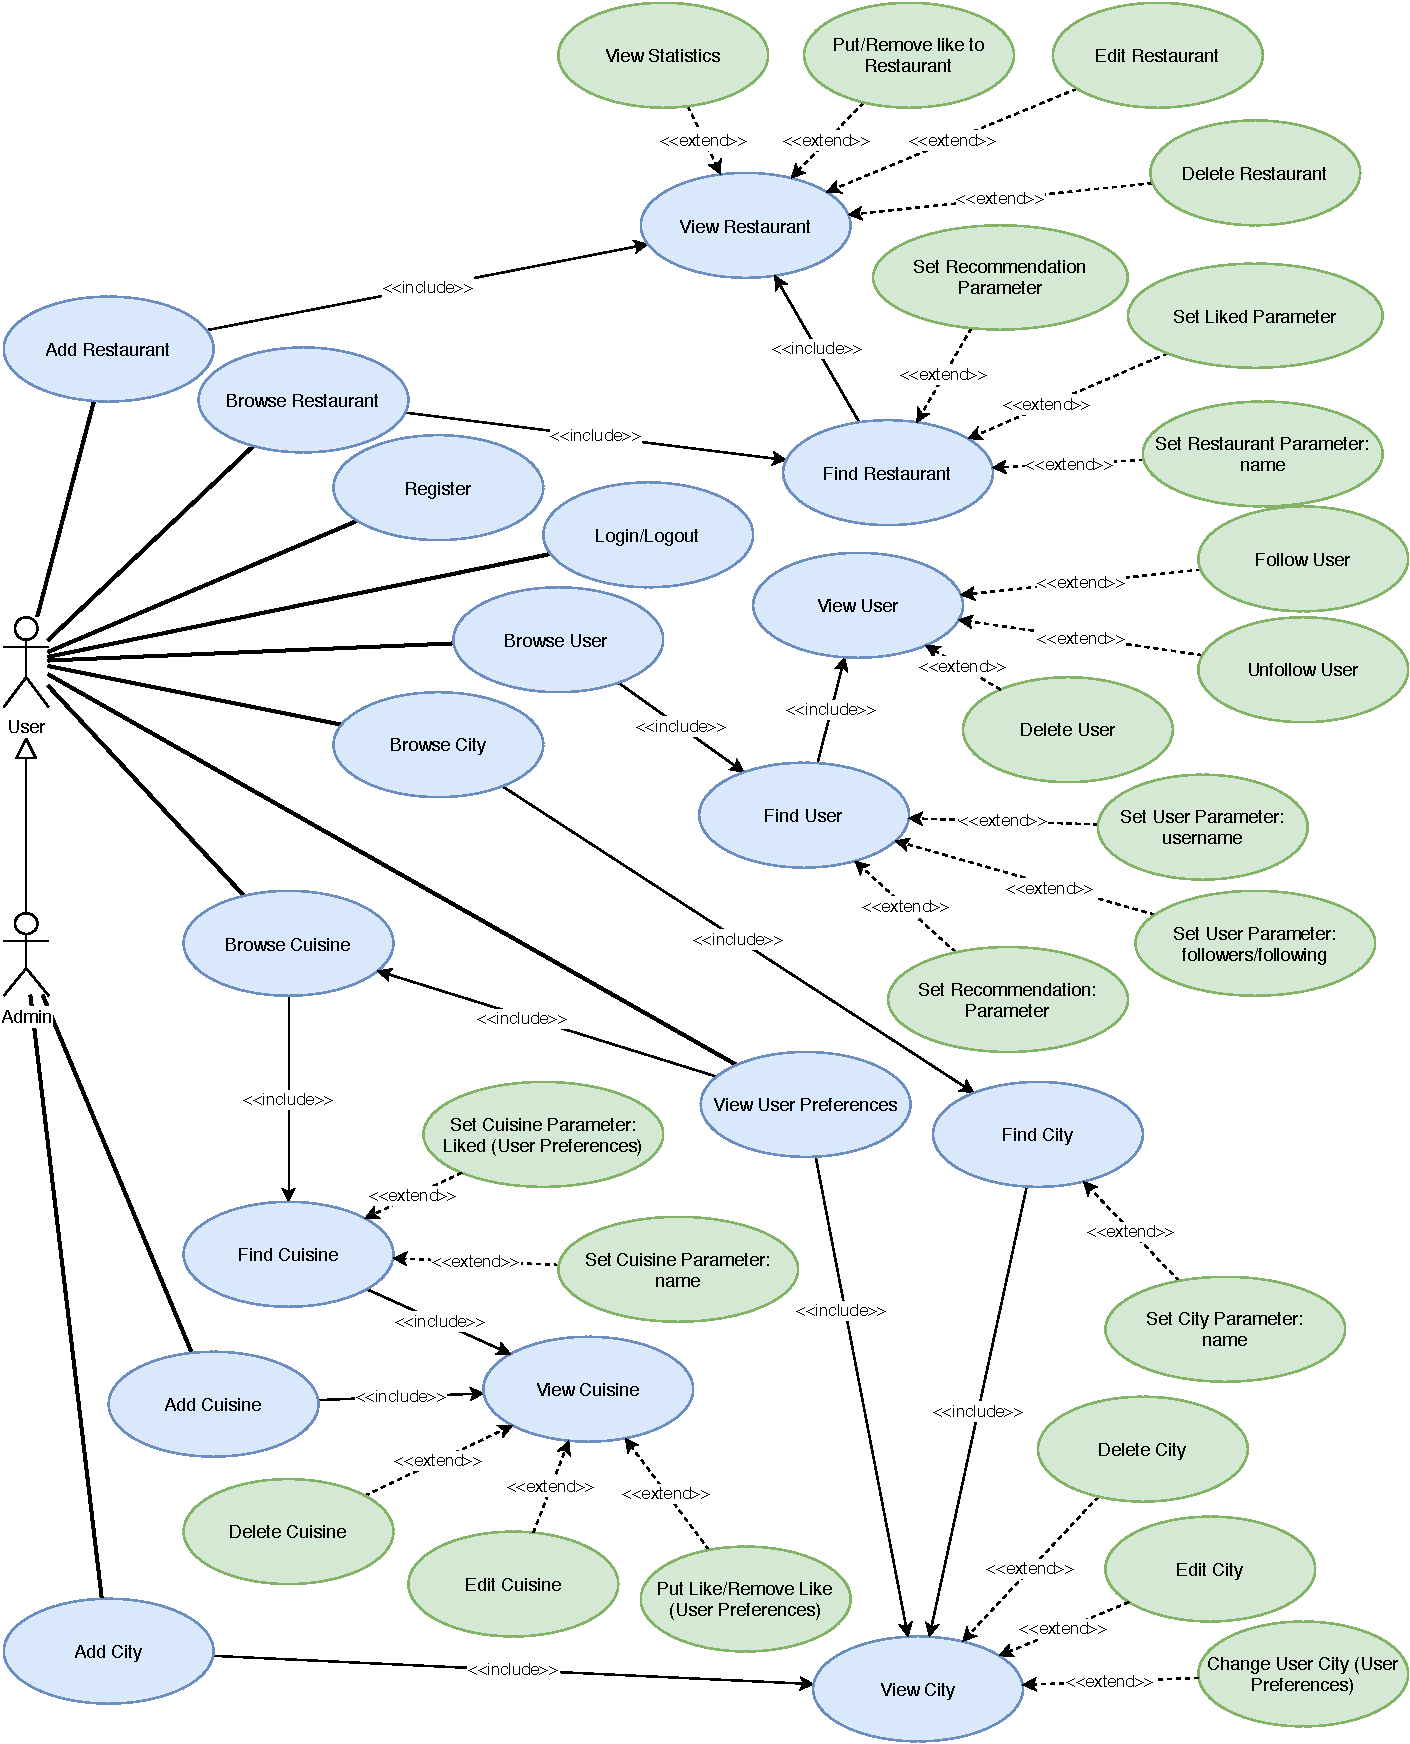
\includegraphics[width=\textwidth]{usecases}
	\caption{Use cases UML diagram.}\label{fig:usecases}
\end{figure}

The following use cases are defined (all use cases, except Login, requires
the user to be logged in):
\begin{description}
	\item[Login/Logout] A user can login in the application using its
		credentials (username, password). When logged in, he can logout
		from the application at any time;
	\item[Register] The first time a user uses the application he/she will
		be asked to register himself/herself, providing an username, a
		password, and the city where he/she lives;
	\item[Browse Restaurant] See the list of all restaurants saved in the
		application;
	\item[Find Restaurant] Search restaurants from the list, searching by
		name or selecting by recommendations parameters;
	\item[View Restaurant] See all the information about a restaurant;
	\item[Put/Remove like Restaurant] a customer can put or remove likes to
		restaurants;
	\item[View Statistics] View the statistics of the restaurant, as
		the  restaurant’s likes and how restaurant is ranked in the
		city where it is located;
	\item[Add Restaurant] Add a new restaurant, providing name,
		cuisine that it serves, price range, city where is located and
		description;
	\item[Delete Restaurant] A user can delete a restaurant if it owns it.
		Moreover, the administrator can delete any user;
	\item[Edit Restaurant] Modify the details of a restaurant;
	\item[Browse User] See the list of all users saved in the application;
	\item[Find User] Search users from the list, searching by name or
		selecting by recommendations parameters;
	\item[View User] See all the information about a user;
	\item[Follow User] A customer can start to follow another customer;
	\item[Unfollow User] A customer can stop to follow another customer;
	\item[Delete User] \textit{(admin)} Remove a user from the system;
	\item[Browse City] See the list of all cities saved in the application;
	\item[Find City] Search cities from the list, searching by name;
	\item[View City] See all the information about a city;
	\item[Add City] \textit{(admin)} Add a new city, providing name,
		latitude and longitude where it is located;
	\item[Delete City] \textit{(admin)} Delete a city among those available
		in the application;
	\item[Change User City] A user can change his/her city where he/she
		lives;
	\item[Browse Cuisine] See the list of all cuisines saved in the
		application;
	\item[Find Cuisine] Search cuisines from the list, searching by name;
	\item[View Cuisine] See all the information about a cuisine;
	\item[Put/Remove like to Cuisine] a customer can put or remove likes to
		cuisines;
	\item[Add Cuisine] \textit{(admin)} Add a new cuisine, providing its
		name;
	\item[Delete Cuisine] \textit{(admin)} Delete a cuisine among those
		available in the application;
	\item[View User Preferences] Show the preferences of a user \idest{the
		city where the user lives and the cuisines she/he likes};
	\item[Change User City]  Change the city where a user lives;
\end{description}

The \textit{Restaurant Recommendation Parameters} allow to select restaurants
that the customer does not known by number of friends' likes, by the city in
which they are located (or by the distance from the city where the customer
lives), by the cuisine they offer and by the price. This is done by running the
query defined in~\secref{sec:restrecommend}.

The \textit{User Recommendation Parameters} allow to select users not followed
by the customer by filtering them by the city in which they live (or by the
distance from the city where the customer lives) and the types of cuisine they
like. This is done by running the query defined in~\secref{sec:userrecommend}.

The \emph{Find City} and \emph{Find Cuisine} use cases include the case when the
user must select a city/cuisine \exgratia{when filling a form} and the
application gives the user suggestions on the available cities and cuisines.
